\section{Relaciones}


	{Ejemplos de relaciones}
	\begin{itemize}
		\item ``menor que''
		\item ``es paralelo a''
		\item ``es un subconjunto de''
	\end{itemize}
	



	Formalmente, definiremos una relación en t\'erminos de \emph{pares ordenados.}



	\begin{defn}
		Un \emph{par ordenado} de elementos $a$ y $b,$ donde $a$ es el primer elemento y $b$ es el segundo se denota por $(a,b).$
	\end{defn}
	



	
	\begin{ax}
		$(a,b)=(c,d)$  si y sólo si $a=c$ y
		$b=d.$
	\end{ax}
	
	
	
	En particular $(a,b)\neq(b,a),$  al menos que $a=b.$
	
	
	
	Esto es muy diferente al caso de un conjunto, dónde el orden es irrelevante:
	$$
	\set{a,b}=\set{b,a}.
	$$


\subsection{Producto de conjuntos}


	Consideremos dos conjuntos arbitrarios $A$ y $B.$ El conjunto de todos los pares ordenadors $(a,b)$ donde $a\in A, b \in B$ es llamado \emph{producto(cartesiano)} de $A$ con $B,$ y se denota por $A \times B,$ es decir,
	$$
	A \times B = \set{(a,b) \mid a \in A, \; b \in B}
	$$



	Podemos construir el producto cartesiano de un conjunto $A$ consigo mismo, y en ese caso denotaremos
	$$A^{2}= A\times A.$$



	\begin{problema}
		Sea $A=\set{x,y}, \, B={0,1}.$ Entonces
		\begin{enumerate}
			\item $A^{2}=\set{(x,x), (x,y), (y,x), (y,y)}$
			\item $A\times B= \set{(x,0), (x,1), (y,0), (y,1)}$
			\item $B\times A= \set{(0,x), (0,y), (1, x), (1,y)}$
			\item $B^2=\set{(0,0), (0,1), (1,0), (1,1)}$
		\end{enumerate}
		
	\end{problema}
	



	\begin{rem}
		\begin{itemize}
			\item En general, $A\times B \neq B \times A.$
			\item Si \emph{$n(A)$} denota el \emph{número de elementos} en el conjunto $A,$ entonces
			$$
			n(A \times B)= n(A) \cdot n(B).
			$$
		\end{itemize}
		
	\end{rem}
	




	Sean $A=\set{1,2}$ y $B={a,b,c}.$ Determine $A\times B,$ $B\times A$ y $A^{2},$ y describa gráficamente estos productos.



	\begin{problema}
		$\R^{2}=\R \times \R$ es llamado frecuentemente el \emph{plano Cartesiano.}
	\end{problema}
	



	\begin{defn}
		Definimos el producto cartesiano de un número finito de conjuntos $A_{1},...,A_{n}$ como
		$$
		\prod_{i=1}^{n} A_{i}= A_{1} \times \cdots \times A_{n}=\set{\left( a_{1},\dots,a_{n} \right)\mid a_{1}\in A_{1}, \dots, a_{n}\in A_{n}}
		$$
	\end{defn}
	



	\begin{rem}
		De manera análoga al caso $n=2,$ definiremos
		$$
		A^{n}=\prod_{i=1}^{n}A.
		$$
		
		
		Por ejemplo, $\R^{3}$ denota el espacio tridimensional.
	\end{rem}
	


\subsection{Relaciones}


	\begin{defn}
		Sean $A$ y $B$ conjuntos arbitrarios. Una \emph{relación binaria $R$,} o simplemente relación, de $A$ a $B$ es un subconjunto de $A \times B.$
	\end{defn}
	



	Para cada $(a,b)\in A \times B$ alguna de las siguientes condiciones (pero no ambas) es cierta:
	\begin{enumerate}
		\item $(a,b)\in R;$ en cuyo caso diremos que \emph{$a$ está $R-$relacionado con $b$,} y escribiremos $a \rel{R} b.$
		\item $(a,b)\not\in R;$ en cuyo caso diremos que \emph{$a$ no está $R-$relacionado con $b$,} y escribiremos $a \nrel{R} b.$
	\end{enumerate}
	



	Si $R$ es una relación de $A$ en sím mismo, es decir $R \subset A^{2},$ entonces diremos que $R$ es una \emph{relación en $A$.}



	\begin{defn}
		Si $R \subset A \times B$ es una relación, el \emph{domino de $R$} es 
		$$
		\dominio{R}=\set{a\in A\mid (a,b)\in R},
		$$ mientras que la \emph{imagen de $R$} es 
		$$
		\imagen{R}=\set{b\in B\mid (a,b)\in R}.
		$$
	\end{defn}
	


\subsection{Ejemplos}

	Sean $A=\set{1,2,3},$ $B=\subset{x,y,z}$ y $$R=\set{(1,y), (1,z), (3,y)}.$$ Entonce $R$ es una relación de $A$ en $B,$ porque $R \subset A \times B.$
	
	
	Respecto a esta relación, por ejemplo,
	$$
	1\rel{R}y, \; 1\rel{R}z, \; 3\rel{R}y,
	$$ pero 
	$$
	1\nrel{R}x, 2\nrel{R}x, 2\nrel{R}y.
	$$
	
	
	En este caso, $\dominio{R}=\set{1,3}$ e $\imagen{R}=\set{y,z}.$



	La propia inclusión $\subset$ es una relación en una colección de conjuntos $A_{1},...,A_{n}.$ 
	
	Para cualquier par $A_{i}, A_{j}$ en dicha colección $A \subset B$ o $A \not\subset B.$



	Una relación en el conjunto $\Z$ de número enteros es \emph{\texttt{``$m$ divide a $n.$''}}
	
	
	La notación convencional para esta relación es \emph{$m \mid n.$}



	Consideremos el conjunto de lineas $L$ en el plano. La perpendicularidad $\perp$ es una relación en $L.$  De manera similar el paralelismo $\parallel.$



	Sea $A$ cualquier subconjunto. Una relación importante en $A$ es la \emph{igualdad}
	$$
	\set{(a,a) \mid a \in A}
	$$ que usualmente se denota por \emph{$$``=''$$} 
	 En ocasiones, tambi\'en se le llama \emph{entidad} o \emph{diagonal} y se denota por $\triangle_{A},$ o simplemente por $\triangle.$



	Sea $A$ un conjunto arbitrario. Entonces tanto $A\times A$ como $\emptyset$ son subconjuntos de $A \times A,$ y son llamados \emph{relación universal} y \emph{relación vacía,} respectivamente.



	{Relación inversa}
	
	Sea $R$ una relación de $A$ en $B.$ La \emph{relación inversa} de $R,$ denotada por \emph{$R^{-1}$,} es la relación de $B$ en $A$ que consiste en todos aquellos pares que al invertirlos, pertenecen a $R.$ 
	
	En otras palabras
	$$
	R^{-1}=\set{(b,a)\mid (a,b)\in R}.
	$$



	\begin{problema}
		Sea $A=\set{1,2,3}, B=\set{x,y,z}$ y $R=\set{(1,y),(1,z),(3,y)}.$ Entonces
		$$
		R^{-1}=\set{(y,1), (z,1), (y,3)}.
		$$
	\end{problema}



	\begin{rem}
		\begin{itemize}
			\item $\left( R^{-1} \right)^{-1}=R.$
			\item $\dominio{R^{-1}}=\imagen{R}$
			\item $\imagen{R^{-1}}=\dominio{R}$
		\end{itemize}
	\end{rem}




\subsection{Composición de Relaciones}

	Sean $A,B,C$ conjuntos arbitrarios, $R$ una relación de $A$ en $B$ y $S$ una relación de $B$ en $S.$  Entonces podemos definir una nueva relación de $A$ en $C$ denotada por \emph{$RS$:}
	\begin{center}
		$a\rel{{RS}}c$ si para alguna $b \in B,$ $a\rel{R}b$ y $b\rel{S}c.$
	\end{center} 



	Esto es
	$$
	RS=\set{(a,c)\mid \exists b\in B: (a,b)\in R, (b,c)\in S}
	$$



	Supongamos que $R$ es una relación en $A.$ Entonces, definimos $R^{n}$ de manera recursiva
	$$
	R^{1}=
	\begin{cases}
		R & n=1 \\
		R^{n-1}R & n>1
	\end{cases}
	$$



	\begin{problema}
		Sea $A=\set{1,2,3,4},$ $B=\set{a,b,c,d}$ y $C=\set{x,y,z}$ y definimos las relaciones: 
		$$R=\set{(1,a),(2,d),(3,a),(3,b),(3,d)}$$  $$S=\set{(b,x),(b,z),(c,y),(d,z)}.$$ Encuentre $RS.$
	\end{problema}
	



	\begin{thm}
		Supongamos que $R$ es uan relación de $A$ en $B,$ y $S$ una relación de $B$ en $C.$ Entonces
		$$
		(RS)T=R(ST).
		$$
	\end{thm}
	


\subsection{Tipos de relaciones}

\subsection{Relaciones reflexivas}


	
	Una relación $R$ es un conjunto $A$ es \emph{reflexiva} si $a\rel{R}a$ para todo $a\in A$, \, es decir, $\forall a \in A: (a,a)\in \R.$ 
	
	Entonces, $R$ es \emph{no-reflexiva} si...



	\begin{problema}
		\label{lip:exmp:2.5}
		Sea $A=\set{1,2,3,4}.$ Determine cuales de las siguientes relaciones son reflexivas:
		\begin{itemize}
			\item $R_{1}=\set{(1,1),(1,2),(2,3),(1,3),(4,4)}$ 
			\item $R_{2}=\set{(1,1),(1,2),(2,1),(2,2),(3,3),(4,4)}$ 
			\item $R_{3}=\set{(1,3),(2,1)}$
			\item $R_{4}=\emptyset$
			\item $R_{5}=A \times A$
		\end{itemize}
		
	\end{problema}
	



	\begin{problema}
		\label{lip:exmp:2.6}
		Determine cuales de las siguientes relaciones son reflexivas:
		\begin{itemize}
			\item $\leq$ en $\Z$ 
			\item $\subset$ en $2^{A}$ 
			Aquí $A$ es un conjunto y $2^{A}$ es la colección de todos sus subconjuntos (incluyendo tanto a $\emptyset$ como $A$) 
			\item $\perp$ en el conjunto $L$ de líneas en el plano 
			\item $\parallel$ en el conjunto $L$ de líneas en el plano 
			\item $\mid$ (divisivilidad) en $\N.$  Aquí $a\mid b$ significa que \emph{a divide a b.} 
		\end{itemize} 
	\end{problema}


\subsection{Relaciones sim\'etricas y antisim\'etricas}


	Una relación $R$ en un conjunto $A$ es sim\'etrica si: Siempre que $a\rel{R}b,$ entonces $b\rel{R}a.$  En otras palabras, 
	$$
	(a,b)\in \R \onlyif (b,a)\in \R.
	$$
	
	Entonces, una relación $R$ no es sim\'etrica si...
 


	\begin{problema}
		\label{lip:exmp:2.7}
		\begin{enumerate}
			\item   Determine cuales de las relaciones en el ejemplo \ref{lip:exmp:2.5} son sim\'etricas.
			\item Determine cuales de las relaciones en el ejemplo \ref{lip:exmp:2.6} son sim\'etricas.
		\end{enumerate}
		
	\end{problema}




	Una relación $R$ en un conjunto $A$ es antisim\'etrica si: Siempre que $a\rel{R}b$ y $b\rel{R}a$ entonces $a=b.$  En otras palabras, 
	$$
	a\neq b, a\rel{R}b \onlyif b\nrel{R}a.
	$$
	
	Entonces, una relación $R$ no es sim\'etrica si...
 


	\begin{problema}
		\label{lip:exmp:2.8}
		\begin{enumerate}
			\item   Determine cuales de las relaciones en el ejemplo \ref{lip:exmp:2.5} son antisim\'etricas.
			\item Determine cuales de las relaciones en el ejemplo \ref{lip:exmp:2.6} son antisim\'etricas.
		\end{enumerate}
		
	\end{problema}



	\begin{rem}
		Las propiedades de simetría y antisimetría no son excluyentes una de la otra. 
		
		Por ejemplo, la relación $$R=\set{(1,3),(3,1),(2,3)}$$ no es sim\'etrica ni antisim\'etrica. 
		
		Por otro lado, la relación $$S=\set{(1,1),(2,2)}$$ es tanto sim\'etrica como antisim\'etrica.
	\end{rem}
	


\subsection{Relación transitiva}


	Una relación $R$ en un conjunto $A$ es transitiva si: Siempre que $a\rel{R}b$ y $b\rel{R}c,$ entonces $a\rel{R}c.$  En otras palabras, 
	$$
	(a,b)\in R, (b,c)\in R \onlyif (a,c)\in \R.
	$$
	
	
	Entonces $R$ no es transitiva si...



	\begin{problema}
		\label{lip:exmp:2.9}
		\begin{enumerate}
			\item   Determine cuales de las relaciones en el ejemplo \ref{lip:exmp:2.5} son transitivas.
			\item Determine cuales de las relaciones en el ejemplo \ref{lip:exmp:2.6} son transitivas.
		\end{enumerate}
		
	\end{problema}


% \subsection{Propiedades de cerradura}
% 
% 
% Consideremos un conjunto dado $A$ y la colección de todas las relaciones en $A,$ y sea $P$ una propiedad en la colección de tales relaciones, por ejemplo, la simetría o la transitividad.
% 
% 
% Si una relación satisface la propiedad $P,$ diremos que es una $P-$relación.
% 

\subsection{Relaciones de Equivalencia}

	Considere un conjunto no-vacío $S.$ Una relación $R$ en $S$ es una \emph{relación de equivalencia} si $R$ es reflexiva, sim\'etrica y transitiva.



	En otras palabras, $R$ es una \emph{relación de equivalencia} en $S$ si satisface las siguientes propiedades:
	\begin{enumerate}
		\item Para cada $a\in S:$ $a\rel{R}a;$
		\item si $a\rel{R}b,$ entonces $b\rel{R}a;$
		\item si $a\rel{R}b,$ $b\rel{R}c,$ entonces $a\rel{R}c.$
	\end{enumerate}
	



	La idea general detras de una relación de equivalencia que es una clasificación de objetos que son en cierto sentido \emph{similares.} 
	
	
	Por ejemplo, la relación \emph{$=$} de igualdad en cualquier conjunto $S$ es una relación de equivalencia, porque...



	\begin{problema}
		\label{lip:exmp:2.12.a}
		Sea $L$ el conjunto de líneas en el plano cartesiano y $T$ el conjunto de triangulos en el mismo plano.
		
		\begin{enumerate}
			\item La relación de paralelidad es una relación de equivalencia en $L;$ 
			\item La relación de congruencia o la de similaridad son relaciones de equivalencia en $T.$
		\end{enumerate}
		
	\end{problema}
	



	\begin{problema}
		\label{lip:exmp:2.12.b}
		La relación $\subset$ no es una relación de equivalencia. Aunque es reflexiva y transitiva,  no es sim\'etrica...
	\end{problema}
	



	\label{lip:exmp:2.12.c}
	Sea $m$ un entero positivo fijo. Dos enteros $a,b$ son llamados \emph{congruentes módulo $m,$} si $m$ divide la diferencia $a-b,$ y en tal caso escribimos:
	$$
	a\equiv b \mod m.
	$$
	
	
	Por ejemplo $11\equiv 3 \mod 4$ y $22\equiv 6 \mod 4.$
	
	
	La relación de congruencia módulo $m$ es un relación de equivalencia. 



\subsection{Particiones y clases de equivalencia}


	Una paritición $P$ de un conjunto no-vacío $S$ es una colección $\set{A_{j}}$de subconjuntos no-vaciós de $S$ con las siguientes propiedades de que cada $a\in S$ pertenece a uno y solo uno de los conjunto $A_{j}$ de la partición.  
	
	En otras palabras,
	\begin{enumerate}
		\item Cada $a\in S$ pertenece a algún $A_{j};$
		\item si $A_{i}\neq A_{j},$ entonces $A_{j}\cap A_{j}=\emptyset.$
		
	\end{enumerate}
	
	
	De manera equivalente, una partición $P$ de $S$ es una subdivisión de $S$ en conjuntos disjuntos no vacíos $A_{j}$ tal que $$S= \sqcup_{j} A_{j}.$$



	Supontamos que $R$ es una relación de equivalencia en el conjunto $S.$ Para cada $a\in S,$ denotemos por $[a]$ el conjunto de elementos de $S$ tales que están $R-$relacionados con $a.$ 
	
	
	En otras palabras,
	$$
	[a]=\set{x \in S \mid (a,x)\in R}.
	$$



	La colección de clases de equivalencia de elementos de $S$ bajo una relación de de equivalencias $R$ se denota por $S/R,$ es decir,
	$$
	S/R=\set{[a] \mid a \in S}.
	$$
	 
	
	Diremos que $S/R$ es el conjunto cociente de $S$ por $R.$



	\begin{thm}
		\label{lip:thm:2.6}
		Sea \emph{$R$ una relación de equivalencia en $S.$} Entonces \emph{S/R es una partición de $S.$} 
		De manera especifica:
		\begin{enumerate}
			\item Para cada $a \in S:$  $a\in [a];$
			\item $[a]=[b]$ si y solo si $(a,b)\in R;$
			\item Si $[a]\neq [b],$ entonces $[a]$ y $[b]$ son conjuntos disjuntos. 
		\end{enumerate}
		
		
		De manera inversa, dada una partición $P=\set{A_{j}}$ de conjuntos $S,$ existe una relación $R$ en $S$ tal que los conjuntos $A_{j}$ son las clases de de equivalencia de $R.$
	\end{thm}
	



	\begin{problema}
		\label{lip:exmp:2.13.b}
		Sea $R=\set{(1,1),(1,2),(2,1),(2,2),(3,3)}$ en $S=\set{1,2,3}.$ Demuestre que $R$ es una relación de equivalencia y calcule $S/R.$
	\end{problema}
	



	\begin{problema}
		Para cada relación, verifique que se trata de una relación de equivalencia, y calcule sus clases de equivalencia.
	\end{problema}
	
	\begin{itemize}
		\item $\displaystyle R_{0}= \left[\left[\text{\texttt{a}}, \text{\texttt{a}}\right], \left[\text{\texttt{b}}, \text{\texttt{b}}\right], \left[\text{\texttt{c}}, \text{\texttt{c}}\right]\right] $
		\item $\displaystyle R_{1}= \left[\left[\text{\texttt{a}}, \text{\texttt{a}}\right], \left[\text{\texttt{a}}, \text{\texttt{b}}\right], \left[\text{\texttt{b}}, \text{\texttt{a}}\right], \left[\text{\texttt{b}}, \text{\texttt{b}}\right], \left[\text{\texttt{c}}, \text{\texttt{c}}\right]\right] $
		\item $\displaystyle R_{2}= \left[\left[\text{\texttt{a}}, \text{\texttt{a}}\right], \left[\text{\texttt{a}}, \text{\texttt{c}}\right], \left[\text{\texttt{b}}, \text{\texttt{b}}\right], \left[\text{\texttt{c}}, \text{\texttt{a}}\right], \left[\text{\texttt{c}}, \text{\texttt{c}}\right]\right] $
		\item $\displaystyle R_{3}= \left[\left[\text{\texttt{a}}, \text{\texttt{a}}\right], \left[\text{\texttt{b}}, \text{\texttt{b}}\right], \left[\text{\texttt{b}}, \text{\texttt{c}}\right], \left[\text{\texttt{c}}, \text{\texttt{b}}\right], \left[\text{\texttt{c}}, \text{\texttt{c}}\right]\right] $
		\item $\displaystyle R_{4}= \left[\left[\text{\texttt{a}}, \text{\texttt{a}}\right], \left[\text{\texttt{a}}, \text{\texttt{b}}\right], \left[\text{\texttt{a}}, \text{\texttt{c}}\right], \left[\text{\texttt{b}}, \text{\texttt{a}}\right], \left[\text{\texttt{b}}, \text{\texttt{b}}\right], \left[\text{\texttt{b}}, \text{\texttt{c}}\right], \left[\text{\texttt{c}}, \text{\texttt{a}}\right], \left[\text{\texttt{c}}, \text{\texttt{b}}\right], \left[\text{\texttt{c}}, \text{\texttt{c}}\right]\right] $
		
	\end{itemize}
	




\begin{problema}
\label{lip:exmp:2.13.b}
Describa las clases de equivalencia de $\Z \mod 5,$ y verifique que las operaciones
$$
[a]+[b]=[a+b], \; [a]\cdot[b]=[a \cdot b]
$$ están bien definidas.   
\end{problema}





\begin{problema}
Considere el conjunto $S=\set{(a,b)\in \Z^{2}\mid b\neq0}$ y la siguiente relación en este conjunto
$
(a,b)\rel{R}(c,d) \iff ad-bc=0.
$
\end{problema}
\begin{enumerate}
\item Demuestre que $R$ es una relación de equivalencia.
\item Demuestre que $[(a,b)]=[(c,d)]$ para todo $n\in\Z, n \neq 0$
$$
[(a,b)]=[(n\cdot a, n\cdot b)]
$$
\item Demuestre que las operaciones
$$
\begin{cases}
[(a,b)]+[(c,d)]=[(ad+bc,bd)] \\
[(a,b)]\cdot[(c,d)]=[(a\cdot c, b \cdot d)]
\end{cases}
$$ están bien definidas
\item Denote por $\frac{a}{b}$ la clase de equivalencia $[(a,b)]$ y reescriba los resultados anteriores usando esta notación.
\item ?`Qu\'e conjunto de números representa el cociente $S/R.$?
\end{enumerate}



\subsection{Relaciones de orden parcial}


	Una relación $R$ en un conjunto $S$ es llamada \emph{orden parcial} de $S$ en $R$ si es reflexiva, antisim\'etrica y transitiva. 
	
	Un conjunto $S$ con un orden parcial $R$ es llamado \emph{conjunto parcialmente ordenado} o \emph{poset.}



	\begin{problema}
		Para cada una de las siguientes relaciones, verifique que es un orden parcial y dibuje su diagrama de Hasse.
	\end{problema}
	\begin{itemize}
		\item $\displaystyle R_{1}= \left[\left[\text{\texttt{a}}, \text{\texttt{a}}\right], \left[\text{\texttt{b}}, \text{\texttt{b}}\right], \left[\text{\texttt{c}}, \text{\texttt{c}}\right]\right] $
		\item $\displaystyle R_{2}= \left[\left[\text{\texttt{a}}, \text{\texttt{a}}\right], \left[\text{\texttt{a}}, \text{\texttt{b}}\right], \left[\text{\texttt{b}}, \text{\texttt{b}}\right], \left[\text{\texttt{c}}, \text{\texttt{c}}\right]\right] $
		\item $\displaystyle R_{3}= \left[\left[\text{\texttt{a}}, \text{\texttt{a}}\right], \left[\text{\texttt{a}}, \text{\texttt{c}}\right], \left[\text{\texttt{b}}, \text{\texttt{b}}\right], \left[\text{\texttt{c}}, \text{\texttt{c}}\right]\right] $
		\item $\displaystyle R_{4}= \left[\left[\text{\texttt{a}}, \text{\texttt{a}}\right], \left[\text{\texttt{a}}, \text{\texttt{b}}\right], \left[\text{\texttt{a}}, \text{\texttt{c}}\right], \left[\text{\texttt{b}}, \text{\texttt{b}}\right], \left[\text{\texttt{c}}, \text{\texttt{c}}\right]\right] $
		\item $\displaystyle R_{6}= \left[\left[\text{\texttt{a}}, \text{\texttt{a}}\right], \left[\text{\texttt{b}}, \text{\texttt{b}}\right], \left[\text{\texttt{b}}, \text{\texttt{c}}\right], \left[\text{\texttt{c}}, \text{\texttt{c}}\right]\right] $
		\item $\displaystyle R_{7}= \left[\left[\text{\texttt{a}}, \text{\texttt{a}}\right], \left[\text{\texttt{a}}, \text{\texttt{c}}\right], \left[\text{\texttt{b}}, \text{\texttt{b}}\right], \left[\text{\texttt{b}}, \text{\texttt{c}}\right], \left[\text{\texttt{c}}, \text{\texttt{c}}\right]\right] $
		\item $\displaystyle R_{8}= \left[\left[\text{\texttt{a}}, \text{\texttt{a}}\right], \left[\text{\texttt{a}}, \text{\texttt{b}}\right], \left[\text{\texttt{a}}, \text{\texttt{c}}\right], \left[\text{\texttt{b}}, \text{\texttt{b}}\right], \left[\text{\texttt{b}}, \text{\texttt{c}}\right], \left[\text{\texttt{c}}, \text{\texttt{c}}\right]\right] $
	\end{itemize}
	



	\begin{problema}
		\label{lip:exmp:2.14}
		Demuestre para cada par $(S,R),$ el conjunto $S$ es parcialmente ordenado respecto a $R:$
		\begin{enumerate}%[(a)]
			\item $(2^{A}, \subset).$ %Aquí $A$ denota un conjunto arbitrario y $2^{A}$ la colección de todos sus subconjuntos.
			
			\item $(\R, \leq )$
			\item $(\N, \mid).$  Muestre que esto no es cierto para $(\Z, \mid).$
		\end{enumerate}
		
	\end{problema}
	


\subsection{Funciones como relaciones}

\subsection{Funciones, gráficas y relaciones}

	Supongamos que para cada elemento de un conjunto $A,$ asignamos un \emph{único} elemento de un conjunto $B;$ diremos que la colección de tales asignaciones es una \emph{función} de $A$ en $B.$ 
	
	
	En tal caso, denotamos escribimos 
	$$f:A\to B, \; a \mapsto f(a)$$
	donde $f(a)\in B$ es la asignación correspondiente a $a\in A.$



	La conexión entre \emph{funciones} y \emph{relaciones} es la siguiente:
	
	
	Definimos la gráfica de una función $f:A\to B$ como el subconjunto de $A \times B$
	$$
	\Gamma_{f}=\set{(a, f(a)) \mid a \in A}.
	$$
	
	
	% $f:A\to B$ es una función si su gráfica es una relación tal que $$(a,b), (a,b')\in \Gamma_{f} \onlyif b=b'.$$  
	\emph{Observe que $\Gamma_{f}$ es una relación en $A\times B.$}
	
	En este caso, diremos que $a\in A$ es la \emph{varible independiente,} mientras que $b\in B$ es la \emph{variable dependiente.}



	De manera reciproca, una relación $R\subset A \times B$ induce una función si 
	$$
	(a,b), (a,b')\in R \onlyif b=b'.
	$$
	
	
	En tal caso (abusando de la notación), la función está definida por 
	$$
	R:A\to B, \; a \mapsto b:=R(a).
	$$



	Entonce, una relación no induce una función si...



	\begin{problema}
		Considere las siguientes relaciones en $A=\set{1,2,3}$
		\begin{enumerate}[(a)]
			\item $f=\set{(1,3),(2,3),(3,1)}$
			\item $g=\set{(1,2), (3,1)}$
			\item $h=\set{(1,3),(2,1),(1,2),(3,1)}$
		\end{enumerate}
		y determine cuales inducen funciones.
	\end{problema}
	




	El conjunto $A$ es llamado \emph{dominio} de la función, y al conjunto $B$ se le conoce \emph{codominio.}
	
	
	La \emph{imagen} de una función $f:A\to B$ se define como
	\begin{align}
		\imagen{f}&={\color{red} f(A)}\\
		&=\set{b \in B \mid \exists a \in A: b=f(a)}\\
		&=\set{f(a)\in B \mid a \in A}
	\end{align}
	



	Frecuentemente, una función puede expresarse por medio de una fórmula matemática. 
	\begin{problema}
		Consideremos la función que asigna a cada número real su cuadrado. Podemos describir esta función escribiendo
		$$
		f(x)=x^{2} \texttt{ o } x\mapsto x^{2} \texttt{ o } y=x^{2}.
		$$
	\end{problema}



	En el ejemplo anterior, la gráfica de $f:\R \to \R$ esta dada por 
	$$
	\Gamma_{f}=\set{(x,y)\in \R^{2}\mid y=x^{2}}
	$$ y es una parábola.
	
	
	Mientras que la imagen de $f$ esta dada por 
	$$
	f(\R)=\set{x^{2}\mid x\in \R}=\set{y\in \R \mid y\geq 0}.
	$$



	\begin{problema}
		La relación 
		$$
		R=\set{(x,y)\in \R^{2}\mid x^{2}+y^{2}=1}
		$$
		no induce una función.
	\end{problema}
	



	\begin{problema}
		Sea $A$ un conjunto arbitrario. La función $:A \to A$ que asigna a cada elemento $a\in A$ el mismo elemento es llamada \emph{identidad,} usualmente denotada por $\id_{A}$ o simplemente $\id$
		
		
		En otras palabras, la identidad está definida por $$
		\id:A\to A, \; a \mapsto \id(a)=a.
		$$ Observe que
		$$
		\Gamma_{\id_{A}}=\triangle_{A}.
		$$
	\end{problema}
	


% 
% \begin{problema}
%  Supongamos que $S \subset A.$ La \emph{inclusión} de $S$ en $A,$ denotada por $i: S \hookrightarrow A$ esta dada por $i(x)=x.$
% 
% 
% Observe que es la asignación es similar a la identidad, pero el dominio está restringido a $S \subset A.$
% 
% 
% La \emph{restricción} $f\mid_{S}$ de una función $f:A \to B$ a $S \subset A$ esta dada por
% $$
% f\mid_{S}: S \to B, \; x\mapsto f(x).
% $$
% \end{problema}
% 
% 

\subsection{Composición de Funciones}


	Consideremos dos funciones $f:A \to B$ y $g:B \to C.$ Podemeos definir una nueva función $:A \to C$ de la siguiente manera
	$$
	a \mapsto {\color{purple}b=f(a)} \mapsto c=g({\color{purple}b})=g({\color{purple}f(a)}).
	$$
	
	
	La función anterior se conoce como \emph{composición} $g$ con se $f$ se describe de la siguiente manera
	$$
	\begin{cases} 
		{\color{red} g\circ f}:A\to C \\ 
		x \mapsto {\color{purple}g(f(x))}.
	\end{cases}
	$$




\begin{problema}
Sean $f(x)=x^{2}$ y $g(x)=x-3.$ Encuentre 
\begin{enumerate}[(a)]
\item $f\circ g$ 
\item $g\circ f$
\end{enumerate}
\end{problema}




\begin{problema}
Sean $f(x)=\sqrt{x}$ y $g(x)=\sqrt{2-x}.$ Encuentre 
\begin{enumerate}[(a)]
\item $f\circ g$ 
\item $g\circ f$ 
\item $f\circ f$ 
\item $g\circ g$
\end{enumerate}

\end{problema}


% 
% \begin{problema}
%  Si $f:A \to B,$ y $i_{S}:S\hookrightarrow A$ es la inclusión de $S$ en $A$, entonces
%  $$
%  f\mid_{S}= f\circ i_{S}.
%  $$
% \end{problema}
% 


\subsection{Funciones inyectivas, suprayectivas e inversas}


	\begin{defn} Consideremos una función $f:A\to B.$ Diremos que
		\begin{enumerate}[(a)]
			\item $f$ es \emph{inyectiva} o \emph{1:1} si $\displaystyle f(a)=f(a')\onlyif a=a'.$ 
			
			\item $f$ es \emph{suprayectiva} o \emph{sobre} si
			$\displaystyle f(A)=B.$ 
			
			\item $f$ es \emph{biyectiva} o \emph{invertible} si la relación inversa de la gráfica $\Gamma_{f}$ induce una función. 
		\end{enumerate}
		
	\end{defn}



	\begin{prop}
		La función $f:A\to B$ es invertible si y solo si es $1:1$ y sobre.  
		
		En tal caso la relación inversa $R^{-1}$ de $R=\Gamma_{f}$ induce una función denotada por $\displaystyle f^{-1}:B\to A$ tal que
		$$
		\begin{cases}
			f^{-1} \circ f = \id_{A}\\
			f \circ f^{-1} = \id_{B}
		\end{cases}
		$$
	\end{prop}
	



	\begin{problema}
		Considere las siguientes funciones y sus posibles composiciones, y determine si son inyectivas, suprayectivas o biyectivas:
		
		\begin{figure}[h!]
			\centering
			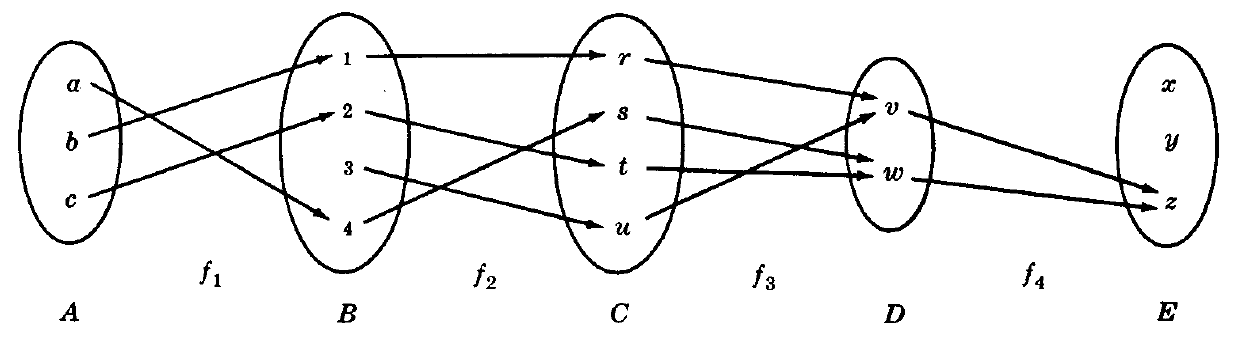
\includegraphics[width=10cm,keepaspectratio=true]{./md/MD02_IM01.png}
			% MD02_IM01.png: 0x0 pixel, 300dpi, 0.00x0.00 cm, bb=
			\label{fig:MD0201}
		\end{figure}
		
	\end{problema}
	



\subsection{Como encontrar funciones inversas}


Si $f:A \to B$ no es \emph{sobre,} es decir, $f(A) \subset B$ pero $f(A)\neq B,$ basta restringir su codominio a la imagen $f(A)$ para que se convierta en {sobre}:
$$
f: A \to f(A).
$$



\begin{problema}
La función $f:\R \to \R, x \mapsto x^{2}$ no es sobre, pero como 
$$f(A)=\set{x^2\mid x\in\R}=\set{y\in \R \mid y\geq 0}$$
la función $f: \R\to \set{y \geq 0}, x \mapsto x^{2}$ sí lo es.
\end{problema}




\begin{figure}[h!]
\centering
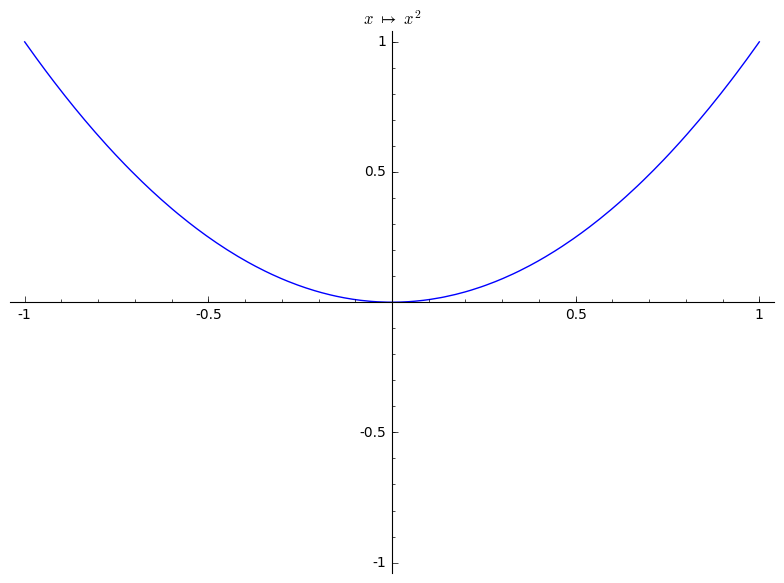
\includegraphics[width=8cm,keepaspectratio=true]{./md/IMG-04_resticcion.png}
% IMG-04_resticcion.png: 0x0 pixel, 300dpi, 0.00x0.00 cm, bb=
\caption{Gráfica de $x^2$}
\label{fig:0401}
\end{figure}




\begin{prop}
Si una función $f:A \to B$ es inyectiva, entonces
$$
f:A \to f(A)
$$ es invertible.
\end{prop}



{Como encontrar la inversa de $y=f(x)$}
\begin{enumerate}[(a)]
\item Verifique que $f(x)$ es un función $1:1.$ 
\item Despeje la variable independiente $y$ en la ecuación $y=f(x)$ para obtener
$$x=f^{-1}(y).$$ 
\item Reescriba la ecuación anterior intercambiando las variables: $y=f^{-1}(x).$
\end{enumerate}




\begin{problema}
Encuentre la inversa de la función $f(x)=3x-2,$
\end{problema}




\begin{problema}
Encuentre la inversa de $f(x)=\dfrac{x^{5}-3}{2}.$
\end{problema}




\begin{problema}
Encuentre la inversa de $f(x)=\sqrt{x-2}.$
\end{problema}




\begin{figure}[h!]
\centering
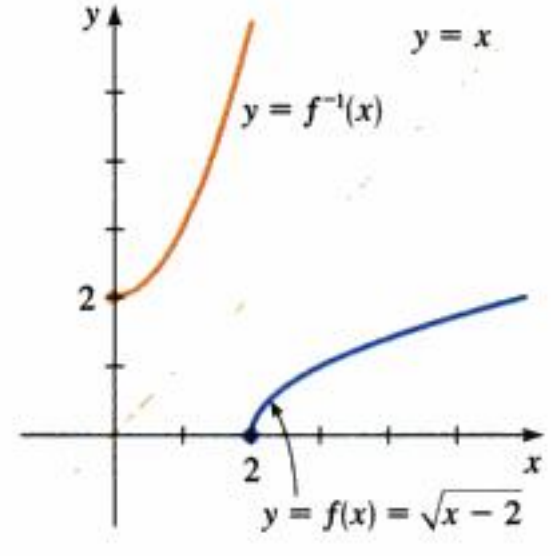
\includegraphics[height=8cm,keepaspectratio=true]{./md/MD02_sqrt_x-2.png}
% MD02_sqrt_x-2.png: 0x0 pixel, 300dpi, 0.00x0.00 cm, bb=
\label{fig:MD02_sqrt_x-2}
\end{figure}


%
\subsection{Caracterización geom\'etrica}


Consiere ahora una función $f:\R \to \R.$ Representemos su gráfica 
$$
\Gamma_{f}=\set{(x,y)\in\R^{2}\mid y=f(x)}
=\set{(x,f(x))}
$$
en el plano.




\begin{rem}
\begin{itemize}
\item $f:\R \to \R$ es \emph{$1:1$} si cada línea \emph{horizontal} intersecta la gráfica de $f$ a lo más en un punto.
\item $f:\R \to \R$ es \emph{sobre} si cada línea horizontal intersecta la gráfica de $f$ al menos en un punto.
\item $f:\R \to \R$ es \emph{invertible} si cada línea horizontal intersecta la gráfica de $f$...
\end{itemize}

\end{rem}



\begin{problema}
Considere las siguientes funciones $:\R \to \R$
\begin{enumerate}
\item $x \mapsto x^{2}$
\item $x \mapsto 2^{x}$
\item $x \mapsto x^{3}-2x^{2}-5x+6$
\item $x \mapsto x^{3}$
\end{enumerate}
y determine si son $1:1,$ sobre o invertibles.
\end{problema}




\begin{figure}[h!]
\centering
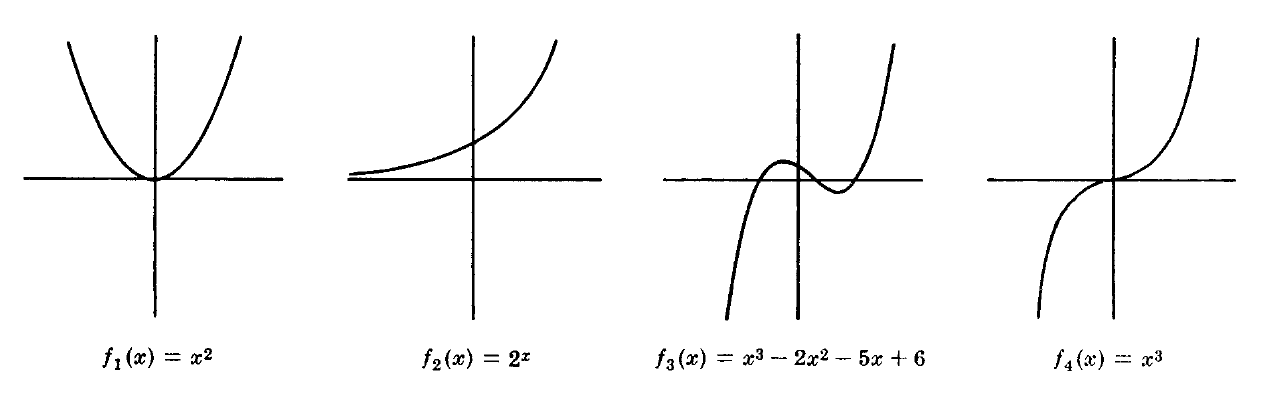
\includegraphics[width=10cm]{./md/MD02_IM02.png}
% MD02_IM02.png: 0x0 pixel, 300dpi, 0.00x0.00 cm, bb=
\label{fig:MD0202}
\end{figure}



\subsection{Permutaciones}


Consideremos un conjunto finito $X=\set{x_{1},...,x_{N}},$ esto es, $X$ tiene \emph{cardinalidad} $n(X)=N < \infty.$


Una función biyectiva (invertible) $\sigma:X \to X$ es llamada \emph{permutación} en $X.$


Observe que las composiciones e inversas de permutaciones, así como la identidad, son tambi\'en permutaciones.


En este caso, diremos que la permutación $\sigma$ \emph{actua} en $X.$



Supongamos que la permutación $\sigma$ actua en $X={x_{1},x_{2},x_{3}}$ de la siguiente manera:
$$
\sigma(x_{1})=x_{2}, \; \sigma(x_{2})=x_{3}, \; \sigma(x_{3})=x_{1}.
$$

Entonces, podemos representar la permitación de la siguiente manera
$$\sigma=
\begin{pmatrix}
1 & 2 & 3 \\
2 & 3 & 1,
\end{pmatrix},
$$  es decir, sólo nos fijamos de que manera actua en el índice $j$ del elemento $x_{j}.$



De manera general, numerando los elemenos de $X=\set{x_{1},...,x_{N}},$ podemos identificar este conjunto con $A_{N}=\set{1,...,N}$ por medio de la biyección $x_{i} \mapsto i.$


Ahora, consideremos una permutación $\sigma:A_{N}\to A_{N},$ tal que $\sigma(i)=\sigma_{i}.$ Entonces podemos representa $\sigma$ por medio de 
$$\sigma=
\begin{pmatrix}
1& ... & N \\
\sigma_{1}& ... & \sigma_{N}.
\end{pmatrix}
$$


El conjunto de todas las permutaciones $:A_{N}\to A_{N}$ se denota por $S_{N}$ y tiene una cardinalidad 
$n(S_{N})=N!.$

